%Choice of research method:
%
%Description: Requirement for 1 point: that the choice of a research strategy and research methods is clearly motivated and described, that alternative research strategies and methods that could be used to solve the research question are discussed, as well as that relevant ethical considerations are discussed. For 2 points the following is also required: that alternative, applicable research strategies and methods are comprehensively discussed and that a profound reasoning about the chosen strategies and methods is made, where the motives for choices made are clearly evident. For 3 points the following is also required: that the choice of method is discussed in relation to the research strategies and methods that are used in current, related research studies that can be regarded as state-of-the-art.
%
%Instructions: It should be evident how the thesis relates to empirical and design research. If the thesis relates to design research then some method framework should be discussed, see for example A Design Science Primer. Research strategies, data collection methods, and data analysis methods should be described. See for example The Good Research Guide for the differences between theses. The description should include references to method literature. There should also be references to literature regarding ethical aspects, for example Appendix 1 in The Good Research Guide. The discussion should be closely tied to the research question of the thesis. There should not be long, general descriptions of research strategies and methods that are only summations from method literature without connections to the thesis topic.
%
%
%
%Application of research method:
%
%Description: Requirement for 1 point: that the application of the chosen scientific strategies and methods are clearly described and that relevant ethical aspects are discussed. For 2 points the following is also required: that the application of research strategies and methods are done in accordance to the demands of said methods and strategies and that a clear argumentation exists for this. For 3 points the following is also required: that there is a real depth to the data analysis
%
%Instructions: How the chosen research strategies and methods (both data collection and data analysis methods) were applied should be clearly described. If the thesis uses design research it should explain how the chosen method framework for design research has been applied. The description should include references to method literature. There should even be references to literature regarding ethical aspects, for example Appendix 1 in The Good Research Guide.



\section{Choice of Research Method}

Empirical research ``aims at describing, explaining and predicting the world''~\cite[Ch. 1]{johannessonPerjons2012}. In comparison, design research additionally wants to improve upon the world through the development of artifacts. This thesis project aims to improve EA by proposing an artifact that can extend the support of existing EA frameworks for decentralization. As a result, a design research approach, specifically design science, will be utilized. The remainder of this section seeks to further demonstrate the suitability of design science and outline the specific research strategies and methods chosen. 

\subsection{Design Science and its Relevance to this Thesis Work}

Design science is concerned with the development and application of \textit{artifacts} aimed at solving some practical problem~\cite{hevner2004,johannessonPerjons2012} in a manner that is of general interest~\cite[Ch. 1]{johannessonPerjons2012}. 

In order to be relevant, Design Science must exist in some context. Johannesson and Perjons~\cite[Ch. 1]{johannessonPerjons2012} define a generic context for design science in terms of people, practices and problems. A practice is a set of related activities performed regularly by people. In the performance of a practice, people encounter practical problems. Two general kinds of problems exist; one where the current state of affairs problematic and the desirable state is neutral, and a second where the current state is neutral and the desirable state is an improvement. The artifacts created through design science can be used by people to solve these practical problems. These concepts are easily related to this thesis work: Enterprise Architecture is a practice with a problem of the second type.  The current state of EA can be seen as being neutral; the problems outlined in this thesis are not necessarily ones that EA practitioners are concerned with.  However, this thesis argues that existing EA frameworks -- each of which can be seen as an artifact composed of smaller artifacts -- can be improved by increased support for decentralization through the development of artifacts addressing the issue of decentralization. 

According to Johannesson and Perjons~\cite[Ch. 1]{johannessonPerjons2012}, artifacts themselves have an ``inner construction'', exist in an environment, and have a function. The inner construction refers to the inner components of the artifact and the relations between them. The environment refers to the artifacts practice, the people using it, and anything else in its surroundings that have an effect on it. Lastly, the function of an artifact is the result of using it in its practice. This definition of an artifact also relates well to this thesis work: the inner construction of our artifact (an EA framework for decentralized organizations) can, at a high level, be seen as an EA method, EA description, and EA engine. The relations for these components are outlined in Figure~\ref{TODO_IRINAS_DIAGRAM}. The environment of our artifact includes the practice of EA and all affected components of the decentralized organization using it, such as involved stakeholders and implementers. The function of our artifact is, on a high level, to bring the benefits of traditional EA to decentralized organizations (e.g. business-IT alignment).

There exist four different types of artifacts: constructs, models, methods, and instantiations~\cite{hevner2004,johannessonPerjons2012}. Enterprise architecture is concerned with the first three of those types: constructs, models and methods. 

\textit{Constructs} are ways to describe some phenomenon. They give a common language for talking about something, but do not make any assertions about reality. For example, the EA description component of an EA framework provides a common taxonomy for the different parts of an organization covered by EA. 

\textit{Models} represent other objects. EA makes use of models, specifically descriptive and prescriptive models. Descriptive models are used to represent a current situation and its challenges, such the ``as-is'' architecture from the EA description. Prescriptive models represent potential future solutions, such as the ``to-be'' architecture, also from the EA description.

\textit{Methods} define ``guidelines and processes for how to solve problems and achieve goals''~\cite[Ch. 1]{johannessonPerjons2012}. The EA method and EA engine  are primarily methods, the former to construct the EA description, the latter to ensure its proper use throughout its lifecycle. 

\subsection{A Design Science Method Framework}
\label{sec:framework}

Having established the relevance of design science to this thesis project, this thesis will therefore follow the framework for a design science method presented by Johannesson and Perjons in ~\cite[Ch. 4]{johannessonPerjons2012}. This method is composed of five activities with input-output relationships: Explicate Problem, Outline Artifact and Define Requirements, Design and Develop Artifact, and Evaluate Artifact. Each activity has an output which serves as an input to the next activity (e.g. an explicated problem is the input to the Outline Artifact and Define Requirements phase). These activities are carried out in an iterative manner, meaning that the practitioner will move back and forth between them as opposed to working in a sequential manner. 

The Explicate Problem activity is concerned with outlining the problem addressed by the research work in detail. To this end, the problem's significance needs to be clearly stated and its underlying causes can be possibly identified and analyzed. The output of this phase an explicated problem. 

The Outline Artifact and Define Requirements activity is where the explicated problem is transformed into the requirements for a solution to said problem. The output of this phase is the set of requirements for the artifact. 

The Design and Develop Artifact activity is where the artifact itself is built based on the requirements for the artifact. The output of this phase is the artifact itself.

The Demonstrate Artifact activity takes the developed artifact and implements it in either a real or illustrative case in order to demonstrate its viability. The output of this phase is the demonstrated artifact. 

The Evaluate Artifact activity is to demonstrate the artifact's fulfillment of the requirements and the degree to which it solves the problem. The output here is an evaluated artifact. 

\subsection{The Role of Research Strategies and Methods in this Design Science Framework}

Each of these activities can make use of controls and resources. Controls are the knowledge used to govern an activity~\cite[Ch. 4]{johannessonPerjons2012}, and  resources are the knowledge used as a basis for the activity. In this method for design science, controls are the research strategies and research methods used. A research strategy is the overall approach used to answer a research question~\cite[Ch. 3]{johannessonPerjons2012}, and research methods are the concrete methods used to generate and analyze data. 


\subsection{Choice of Research Strategy}

Alternative strategies exist for undertaking research in the field of design science. A number of common strategies will be briefly outlined in order to discuss their suitability for this thesis. 

Surveys aim to take a comprehensive look at something by gathering data from a large number of different sources. This data is then analyzed in some manner. Surveys offer a wide view~\cite{denscombe2010good,johannessonPerjons2012}, and as such, are not well suited for a depth view of something. This does not fit in with this project which takes an in-depth look at EA frameworks. 

Experiments employ a controlled and artificial environment in order to isolate a small number of specific factors to study them in detail. The effects of manipulating variables in the environment needs to be precisely measured~\cite{denscombe2010good}. This poses a problem for EA as organizations are highly complex entities where it would be exceptionally difficult to exert precise control and precisely measure the effects. For this reason, experiments are not a suitable strategy for this project. 

In action research, the researcher is an active participant in affecting the environment they are researching. Here, the research is done as part of the practice, as opposed to it being a separate activity~\cite{denscombe2010good}. This could be a highly effective strategy for this thesis topic as it would allow the researcher to experience the problems of decentralization first-hand. Furthermore, action research is a cyclical process, meaning the researcher could repeatedly try out different solutions and evaluate their effects in order to come to a good solution. This would allow for a researcher in a decentralized organization the flexibility to find a solution that works. Despite this fit to the thesis topic, the practical issue of finding a decentralized organization that is willing to go through this process is a significant one. As a result, action research is not used in this project. 

Ethnography is similar to action research in that the researcher becomes a member of the environment being researched. The difference lies in that they are there to integrate themselves into it, rather than affect change~\cite{denscombe2010good}. This could be an applicable research strategy for understanding problems from the perspective of stakeholders, however finding a decentralized organization with some sort of EA (or at least an interest in it) is quite the challenge in itself. Additionally, ethnography requires a large time investment in order to integrate adequately into the environment of study, which is not feasible for a Master's project. For these reasons, ethnography is not used in this project. 

Case studies take an in depth view of a single instance of the practice where the problem of interest exists. Case studies are ideal when ``a researcher wants to investigate an issue in depth and provide an explanation that can cope with the complexity and subtlety of real life situations''~\cite{denscombe2010good}. This project is interested in an in depth view of the problem of suitability of EA for decentralized organizations and decentralized organizations are real life entities that are highly complex. Furthermore, in contrast with ethnography and action research, conducting a single case study fits in well with the scope of a Master's project; it is not necessary for the subject organization to invest large amounts of resources into the project and time investment of a case study fits in with a short-term project. For these reasons, this thesis project will employ a case study research strategy.  

\subsection{Choice of Research Methods}

Research strategies do not prescribe any concrete ways to generate and analyze data. Specific research methods for data generation and data analysis are needed. 


\paragraph*{Data generation methods}

%%data generation

This thesis employs the use of interviews and document studies for data generation.  Document studies are used as a large amount of data on the structure of the organization being studied is available. Documents are a good source of authoritative, objective, and factual data~\cite{denscombe2010good}, which therefore gives a solid foundation on understanding the studied organization. Interviews were chosen in order to supplement this data with information from stakeholders about the organization. Interviews are suited for gaining insight into complex phenomena, which is supportive of our need for an in-depth view of a complex entity that is an organization. Furthermore, interviews are practical for this project as; a) the organization being studied does not need to invest large amounts of time and b) I have physical access to potential interviewees. 

Other common data generation methods are questionnaires and observations. Questionnaires are not particularly suitable for this project as they are most useful when used for specific, straightforward information~\cite{denscombe2010good}. This project, on the other hand, is interested in the complexities of an organization. An observation study would require spending time in an organization in order to directly observe its operations. As this thesis is conducted as an individual project, this is not a feasible activity, due to the size and complexity of an organization.

\paragraph*{Data analysis methods}

After the data has been obtained, it is necessary to analyze it in order to understand the object being studied. Data can be analyzed in either a quantitative or a qualitative manner. Quantitative data analysis is concerned with numeric data, whereas qualitative deals with words and visuals. According to Denscombe ~\cite{denscombe2010good}, some other differences between the approaches are; quantitative research is generally associated with large-scale studies whereas qualitative research is concerned with small-scale studies, and quantitative research is concerned with ``specific variables'' while qualitative research takes a ``holistic perspective''. This project follows a qualitative approach because; a) the data being analyzed will composed of words coming from interviews and document studies, b) this is a small-scale study, and c) this project is interested in a holistic perspective on our case study subject.

\section{Application of Method}

This thesis work follows the framework by Johannesson and Perjons~\cite[Ch. 4]{johannessonPerjons2012} presented above in Section \ref{sec:framework}. This thesis deviates slightly from their proposed framework as the formal ``evaluate artifact'' activity will not be performed. This section will first elaborate on how the different activities will be accomplished and then outline the overall process. 

As suggested in the framework, the IDEF0 notation will be used for visualizing the various activities. In this notation, each activity as an input and output, controls in the form of research strategies and methods, and resources which is the knowledge base for the activity. 

\subsection{Case Study: An Institution of Higher Education in Sweden}
\label{sec:case}

This thesis work will use an institution of higher education in Sweden as an illustrative case study. This case was chosen as an example of a decentralized organization with an implicit EA, i.e., there is no formal EA framework used, but as they use IT extensively, some form of implicit architecture must exist. An advantage of this case is that, as a public institution, many official documents are available on its organizational structure, thus making a document study a viable research method. The documents that formed this study are described in Table~\ref{tab:doc_study}.

A disadvantage of this case is that there is no use of modern EA frameworks in the institution, which weakens the link between the institution and the practice of EA. 

This thesis is not aiming at effecting change in this institution. The focus is instead on: analyzing the state of its EA in order to assess the decentralization support provided in contrast with what is needed; and proposing part of an EA that can provide the needed support. 

\begin{table}  
  \begin{tabular}[c]{| p{\dimexpr 0.4\textwidth-2\tabcolsep} |
                       p{\dimexpr 0.6\textwidth-2\tabcolsep} | }
    \hline
    \textbf{Document} & \textbf{Description} \\
    \hline
    Institution's homepage & Contains descriptions of the different organizational areas of the institution as well its organizational structure \\
    \hline
    Authority delegation documents & These publicly available documents specify authority and delegations of said authority of the institution's organizational units \\
    \hline
    Rule book & The official rule book of the institution detailing rules and decisions that must be followed by the institution \\
    \hline
  \end{tabular}
  \caption{\textbf{Documents forming the document study}}
  \label{tab:doc_study}
\end{table}

Four separate interviews are conducted in order to get a holistic view of the institution. The roles of the interviewees are: vice division lead, head of PhD studies, head of undergrad studies, and head of IT. The interviews are conducted in a semi-structured manner, starting with a set of open-ended questions that promote the interviewees to elaborate on their views. 

%TODO REF TO APPENDIX

\subsection{Research Activities}

\subsubsection*{Iterations Between Activities}

This research is conducted through two general iterations between the research activities:
\begin{description}
  \item[Iteration \#1] The first iteration focuses on using literature for conducting the research activities. In this iteration, the explicate problem activity and the generate sub-activity of design and develop artifact were performed. %In this iteration, the activities explicate problem, outline artifact and define requirements, and the generate sub-activity of design and develop artifact were performed. 
  \item[Iteration \#2] The second iteration focuses on the case study in order to supplement and confirm findings from the first iteration. In this iteration, the activities explicate problem, outline artifact and define requirements, the search-and-select sub-activity of design and develop artifact, and demonstrate artifact were performed.%In this iteration, the activities explicate problem, outline artifact and define requirements, the search-and-select sub-activity of design and develop artifact, and demonstrate artifact were performed.
\end{description}

\subsubsection*{Explicate problem}

Figure \ref{fig:method_problem} outlines the major components of this activity:
\begin{description}
  \item[Sub-activities] Define Precisely, Motivate Problem and Find Root Causes~\cite[Ch. 5]{johannessonPerjons2012}
  \item[Input] The initial problem as described in Section \ref{sec:problem}
  \item[Resources] A literature study on centralization/decentralization in  organizational theory, and on the modern EA frameworks TOGAF, Zachman, and FEA. These three frameworks were chosen due to their popularity and extensive available literature.
  \item[Controls] A case study research strategy that will make use of interviews and a document study. The case is detailed in Section \ref{sec:case}. 
  \item[Output] A fully explicated problem, specifically, the set of specific shortcomings of modern EA frameworks when applied to decentralized organizations determined in the ``find root causes'' sub-activity.
\end{description}

\paragraph{Iteration \#1}

The first sub-activity, Define Precisely, is accomplished with the use of the literature reviews on centralization/decentralization in  organizations and on EA. A classification for decentralization organizations will be built from the literature review for use in the problem definition. 

In the second sub-activity, the problem is motivated through the use a literature review on decentralized organizations. Here, the differences between centralized and decentralized  organizations are specified in order to show that there is a problem. 

The third sub-activity, find root causes, is accomplished through a literature review. An in-depth analysis of each of the three EA frameworks will done to find specific shortcomings; aspects where the framework provides support for centralized organizations and not decentralized organizations. Aspects that are supportive of decentralization will be presented as well.

\paragraph{Iteration \#2}

The first sub-activity, the problem in the case is precisely defined 

In the second sub-activity, the problem is motivated through the use of the case study. To this end, a specific issue in the case that arises from their implicit EA and their organizational structure is identified.

The root causes of these issues are then determined in the third sub-activity. This will be done by developing a lightweight ``as-is'' architecture for the case. 

\begin{figure}
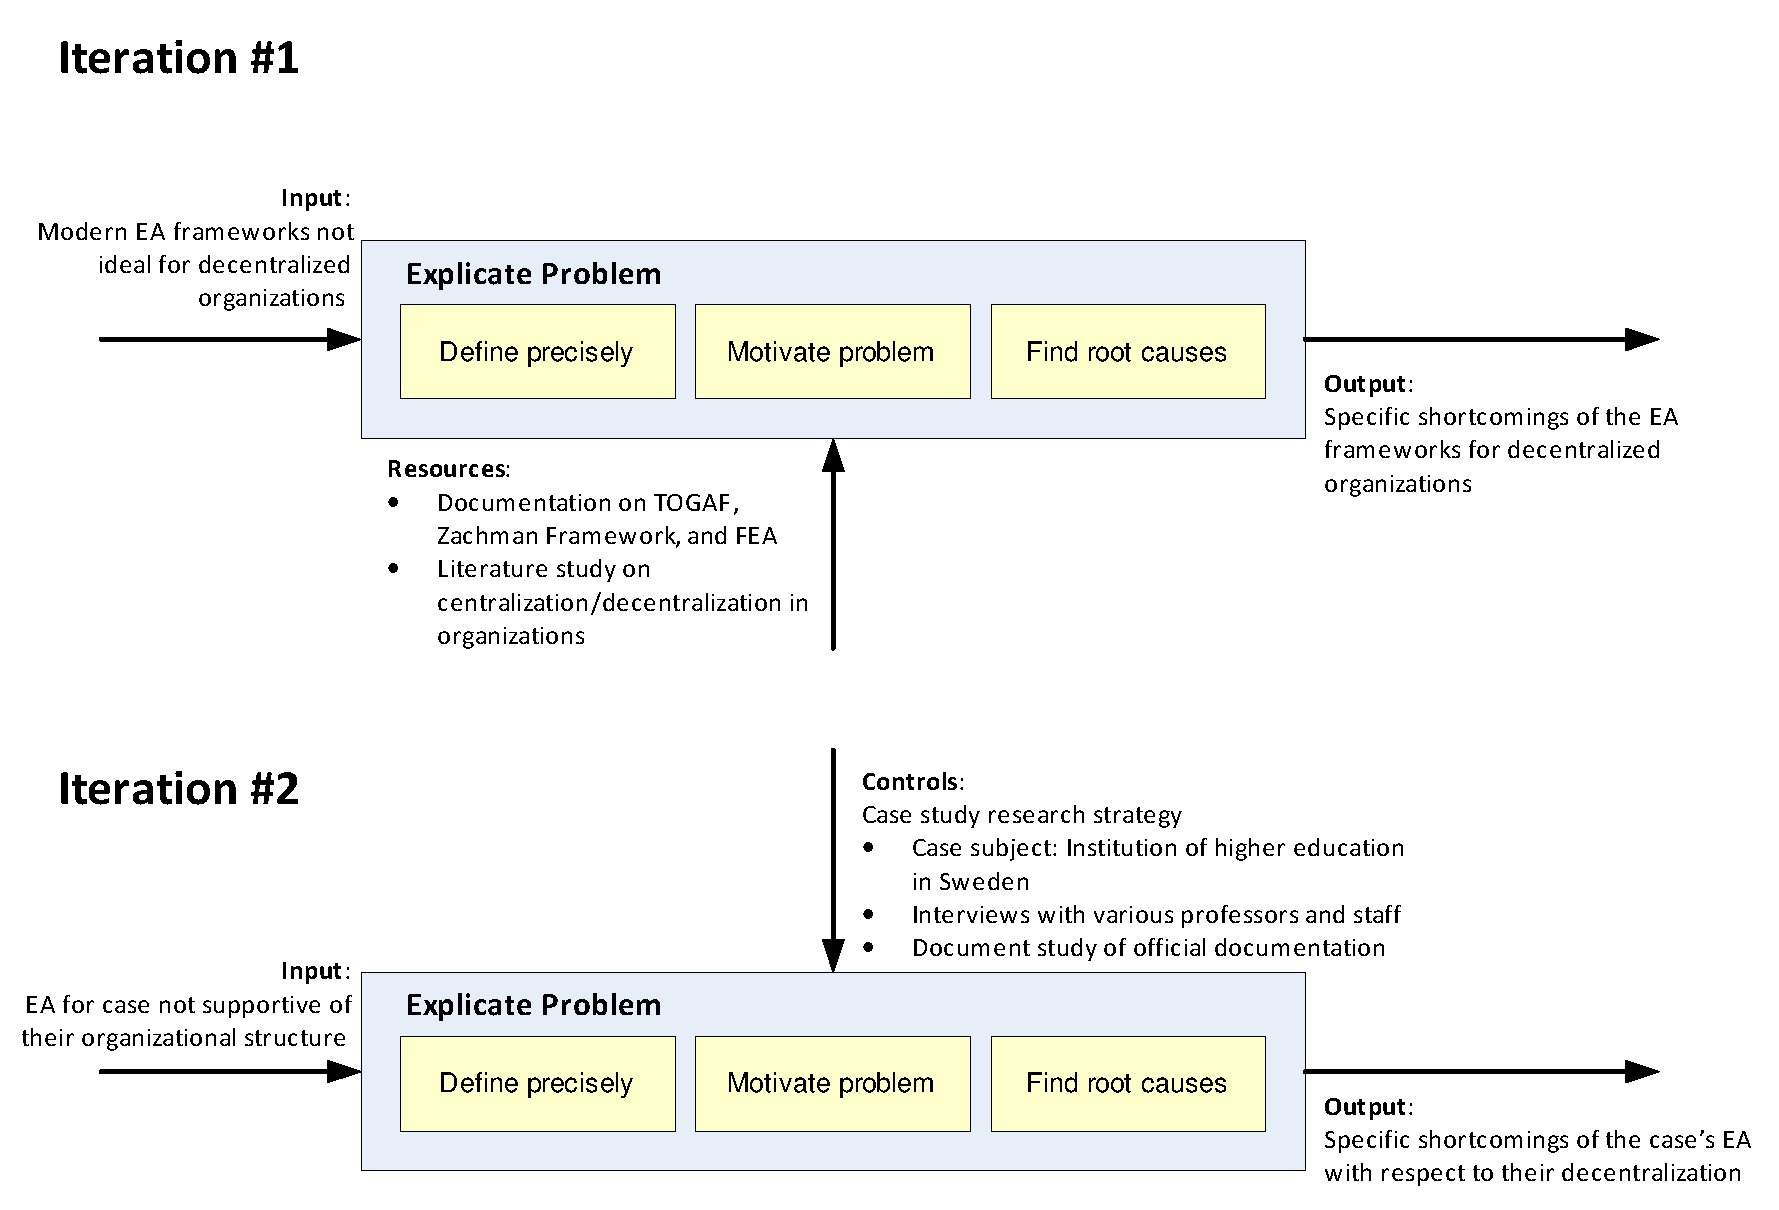
\includegraphics[scale=0.5]{method_problem}
\caption{Explicate problem activity}
\label{fig:method_problem}
\end{figure}

\subsubsection*{Outline artifact and define requirements}

Figure \ref{fig:method_outline} outlines the major components of this activity:
\begin{description}
  \item[Sub-activities] Outline Artifact and Define Requirements~\cite[Ch. 6]{johannessonPerjons2012}
  \item[Input] Set of specific shortcomings of modern EA frameworks when applied to decentralized organizations
  \item[Resources] Literature study on centralization/decentralization in  organizations
  \item[Controls] Case study research strategy
  \item[Output] Requirements for part of a decentralized EA
\end{description}

\paragraph{Iteration \#2}

In the first sub-activity Outline Artifact, the type of artifacts being developed is specified. 

In the second sub-activity, Define Requirements, the requirements for the developed artifact are elicited. This is based on the specific shortcomings of the case's EA, the specific shortcomings of EA frameworks, and on the literature study on centralization/decentralization in organizations.


\begin{figure}
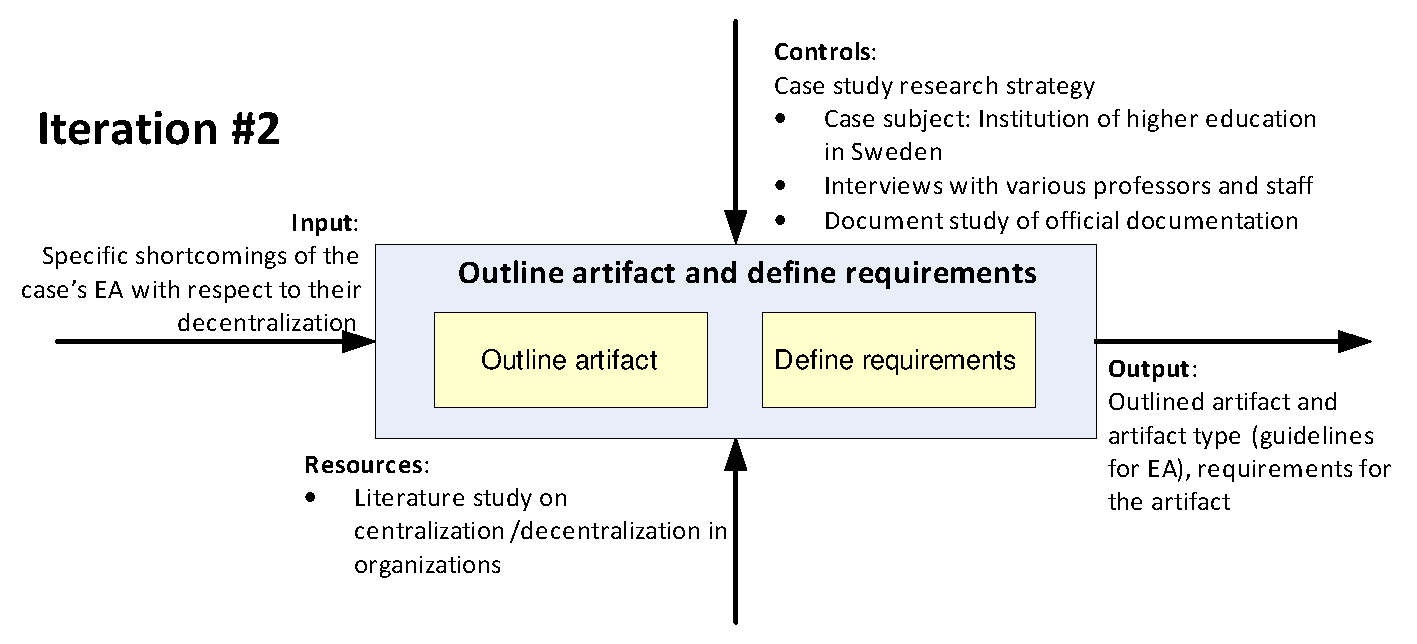
\includegraphics[scale=0.5]{method_outline}
\caption{Outline artifact and define requirements activity}
\label{fig:method_outline}
\end{figure}

\subsubsection*{Design and develop artifact}

Figure \ref{fig:method_design} outlines the major components of this activity:
\begin{description}
  \item[Sub-activities] Generate and Search and Select ~\cite[Ch. 7]{johannessonPerjons2012}
  \item[Input]  Requirements for a decentralized EA 
  \item[Resources] Literature study on peer-to-peer architectures
  \item[Controls] None
  \item[Output] Prototype of one artifact for one aspect of an EA framework for decentralized organizations 
\end{description}

\paragraph{Iteration \#1}

In this iteration, only the Generate sub-activity is performed. Here, a small number of different artifacts that could be potential solutions are outlined. The basis for these artifacts comes from a literature study on peer-to-peer architectures where principles relevant to EA are identified. Peer-to-peer architectures were chosen because they have offered solutions to decentralization in other domains (e.g. technical) and might therefore be able to provide solutions for the practice of EA. 

\paragraph{Iteration \#2}

In this iteration, one of the outlined solutions is selected and elaborated on to create a prototype of one artifact for an EA framework for decentralized organizations. This selection is based on its applicability to the case. 

\begin{figure}
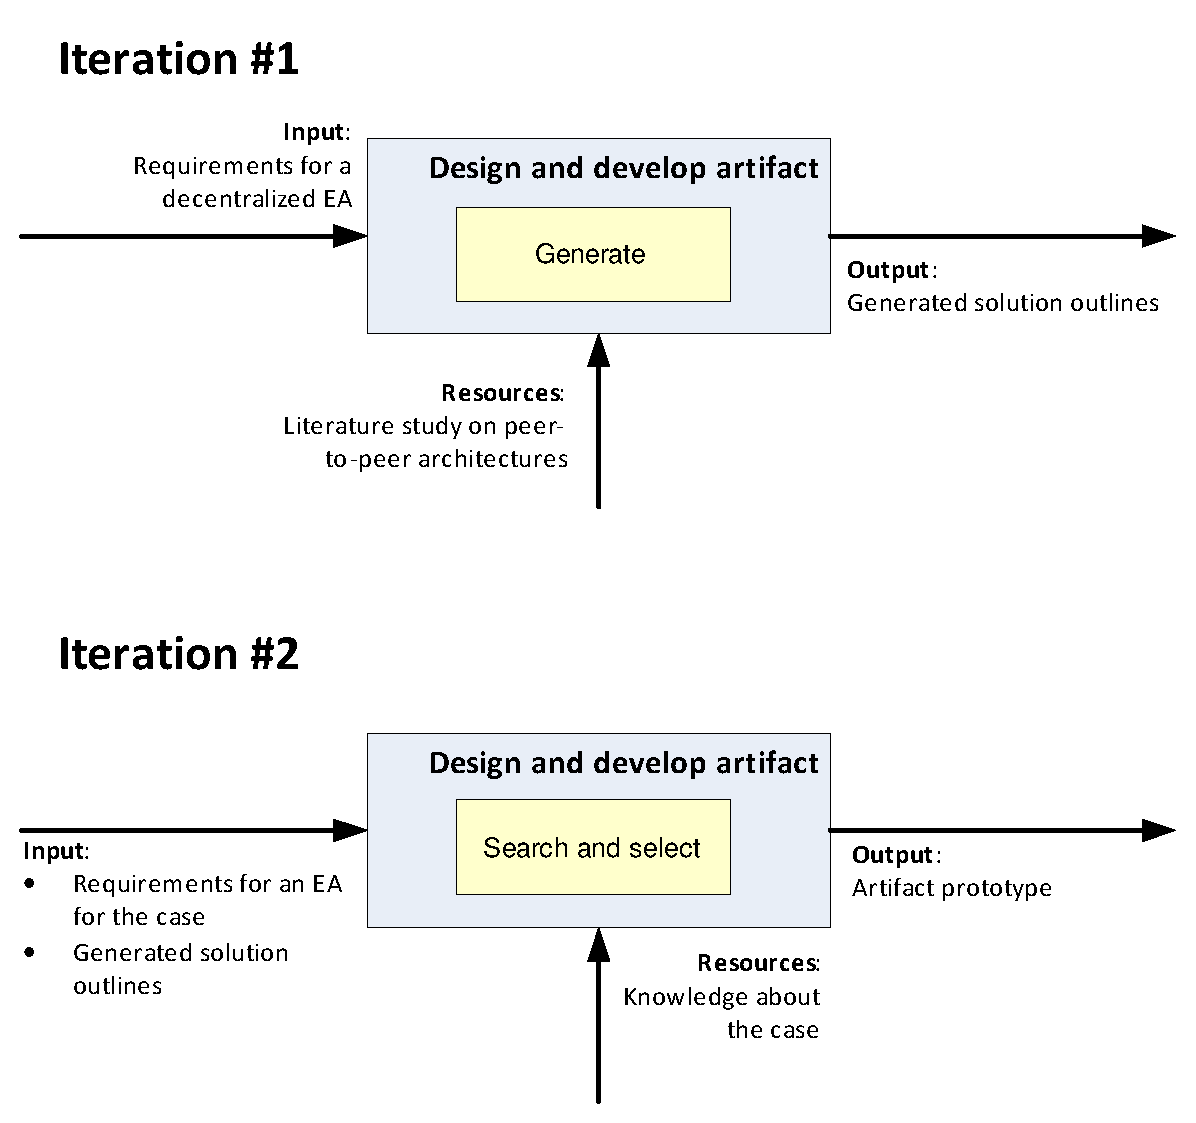
\includegraphics[scale=0.5]{method_design}
\caption{Design and develop artifact activity}
\label{fig:method_design}
\end{figure}
  
\subsubsection*{Demonstrate artifact}

Figure \ref{fig:method_demo} outlines the major components of this activity:
\begin{description}
  \item[Sub-activities]  Choose or Design Case and Apply Artifact~\cite[Ch. 8]{johannessonPerjons2012}
  \item[Input] Prototype of one artifact for one aspect of an EA framework for decentralized organizations
  \item[Resources]  Knowledge on the selected case (institution of higher education in Sweden)
  \item[Controls]  A case study research strategy that will make use of interviews and a document study
  \item[Output] Proof-of-concept artifact for one part of an EA framework prototype
\end{description}

\paragraph{Iteration \#1}

This activity is not performed in the first iteration. 

\paragraph{Iteration \#2}
For the Choose or Design Case sub-activity, an institution of higher education in Sweden has been selected. Details on the case are described in \ref{sec:case}.

In the Apply Artifact sub-activity, the artifact is applied to the case by creating a to-be architecture for the relevant aspect of the case. This to-be architecture is the proof-of-concept artifact for one part of an EA framework prototype.


\begin{figure}
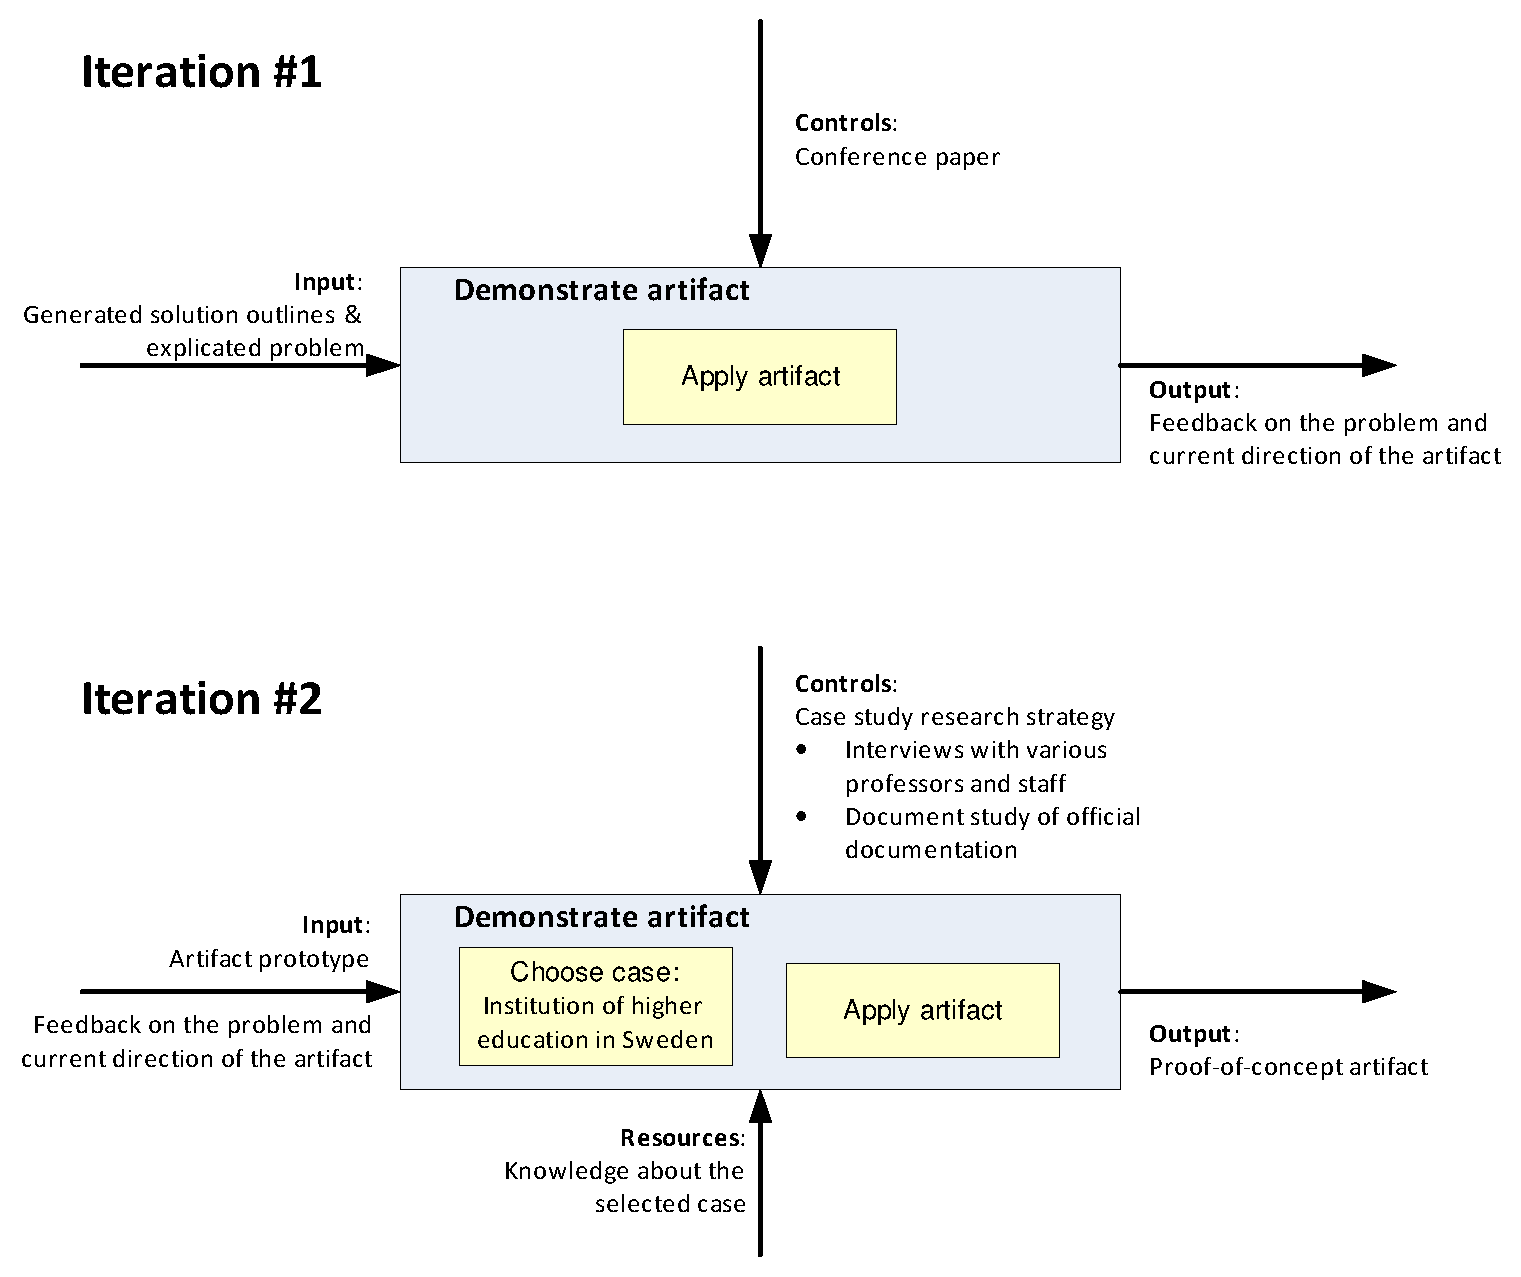
\includegraphics[scale=0.5]{method_demo}
\caption{Demonstrate artifact activity}
\label{fig:method_demo}
\end{figure}

\subsubsection*{Evaluate artifact}

A formal evaluation for the developed artifact would be conducted by actually implementing it in the case and analyzing the results of the implementation. However, the focus of this thesis work is on explicating the problem of decentralization for EA and demonstrating a proof-of-concept of a partial solution. 

\section{Ethical Considerations}

As the proof-of-concept does not involve any actual implementation, the ethical considerations for this research project are minimal and only involve withholding the identity of the case institution. 
